\documentclass[a4paper]{article}
\setlength{\topmargin}{-1.0in}
\setlength{\oddsidemargin}{-0.2in}
\setlength{\evensidemargin}{0in}
\setlength{\textheight}{10.5in}
\setlength{\textwidth}{6.5in}
\usepackage{enumitem}
\usepackage{amsmath}
\usepackage{hyperref}
\usepackage{amssymb}
\usepackage[dvipsnames]{xcolor}
\usepackage{mathpartir}
\usepackage{kbordermatrix}
\usepackage{graphicx}
\usepackage{tikz}
\usepackage{xcolor}
\usepackage{float}
\usetikzlibrary{arrows}
\usetikzlibrary{patterns}
\usepackage{tkz-berge}
\usetikzlibrary{automata, positioning, arrows}

\tikzstyle{arrow} = [thick,->,>=stealth, line width=1.1pt]
\definecolor{lightblue}{rgb}{0.68, 0.85, 0.9} 
\definecolor{lightorange}{rgb}{1, 0.8, 0.6} 
\tikzset{accept/.style = {
    circle, 
    draw=cyan!30!black, 
    thick,
    fill=lightblue,
    inner sep=2pt,
    minimum size=2pt } }
\tikzset{->, node distance=3cm, every state/.style={thick, fill=gray!10},  initial text=$ $,}
\tikzset{uedge/.style = {
    draw=black!8, 
    very thick} }
\tikzset{pathedge/.style = {
    draw=lightorange!300, 
    very thick} }

\tikzset{rede/.style = {
    draw=red!80, 
    very thick} }
\tikzset{bluee/.style = {
    draw=blue!80, 
    very thick} }

\hypersetup{
    colorlinks=true,
    linkcolor=blue,
    filecolor=magenta,      
    urlcolor=cyan,
    pdftitle={Assignment 1},
    pdfpagemode=FullScreen,
}
\def\endproofmark{$\Box$}
\newenvironment{solution}{\par{\bf Solution}:}{\endproofmark\smallskip}
\begin{document}
\begin{center}
    

\vspace{0.1in}

{\large \bf \color{blue}  Notes on Manifolds and Topological Spaces} \\

\vspace{0.05in}

    { \bf \color{YellowOrange} For the LGP REU program 2024}
\end{center}
\medskip

\hfill {\textbf{Name:} Vishnu Varadarajan}

\bigskip
\hrule

\section{Manifolds}
An $n$-dimensional manifold $M$ is a topological space for which 
\[
\forall x \in M, \ x \text{ has an open } \epsilon\text{-ball neighborhood homeomorphic to } \mathbb{R}^n.
\]

\subsection{Topological Space}
\begin{itemize}
    \item $N$ is a topological space if: \\
    Let $X$ be a set, $N: X \to (X^P \setminus \{\emptyset\})^P$.

    $N$ is a topological space if:
    \begin{itemize}
        \item[(i)] $N \in N(x)$ then $x \in N$ \hfill \textit{points}
        \item[(ii)] $x$ belongs to each of its nbhd
        \item[(iii)] $N \in X$ and $N' \subseteq N$ is a nbhd, $N$ is also nbhd. \\
        $N \cap N' \in N(x)$ if $N', N \in N(x)$ \hfill \textit{Neighborhoods}
        \item[(iv)] $N$ induces an $N'$ such that $\forall x \in N'$, $N \in N(x)$
    \end{itemize}
    \item $N$ is also said to be a topological space if:
     \begin{enumerate}
        \item The empty set and the whole set are in $T$:
        \[
        \emptyset \in T \quad \text{and} \quad X \in T
        \]
        
        \item The union of any collection of sets in $T$ is also in $T$:
        If $\{U_i\}_{i \in I}$ is any collection of sets in $T$, where $I$ is an arbitrary index set, then:
        \[
        \bigcup_{i \in I} U_i \in T
        \]
        
        \item The intersection of any finite collection of sets in $T$ is also in $T$:
        If $U_1, U_2, \ldots, U_n \in T$, then:
        \[
        \bigcap_{k=1}^n U_k \in T
        \]
        
        \item A set $X$ equipped with a topology $T$ is called a topological space and is denoted by the pair $(X, T)$.
    \end{enumerate}
\end{itemize}


\subsection{Homeomorphic}
$\exists$ a bijective function between the two topologies. \\
Homeomorphic transformations preserve all the topological properties of a topology.
\subsubsection{Topological Properties}
Homeomorphic invariants are properties of topological spaces that are preserved under homeomorphisms. In other words, if two spaces are homeomorphic, they must share the same values for these properties. Here are some important homeomorphic invariants:

\begin{enumerate}
    \item \textbf{Connectedness} \\
    A topological space $X$ is connected if it cannot be partitioned into two disjoint nonempty open sets. That is, if $X = A \cup B$ where $A$ and $B$ are open sets, and $A \cap B = \emptyset$, then either $A = \emptyset$ or $B = \emptyset$. If two spaces are homeomorphic, one is connected if and only if the other is connected.
    
    \item \textbf{Path-Connectedness} \\
    A space is path-connected if any two points can be joined by a continuous path within the space. Path-connectedness is also a homeomorphic invariant.
    
    \item \textbf{Compactness} \\
    A topological space $X$ is compact if every open cover of $X$ has a finite subcover. That is, if $\{U_i\}_{i \in I}$ is an open cover of $X$, then there exists a finite subset $J \subseteq I$ such that $\{U_j\}_{j \in J}$ is also an open cover of $X$. Compactness is preserved under homeomorphisms, meaning if one space is compact, any space homeomorphic to it must also be compact.
    
    \item \textbf{Hausdorff Condition (T2)} \\
    A space is Hausdorff if any two distinct points have disjoint neighborhoods.
    Formally, a topological space $(X, \tau)$ is Hausdorff if for distinct $x,y \in X$ there exist open sets $U,V \in \tau$ 
    This property is invariant under homeomorphisms.
    
    \item \textbf{Countability Axioms} \\
    \textit{First-Countability}: A space is first-countable if each point has a countable local base (neighborhood basis). \\
    \textit{Second-Countability}: A space is second-countable if its topology has a countable base. \\
    Both first-countability and second-countability are homeomorphic invariants.
    
    \item \textbf{Number of Components} \\
    The number of connected components in a space is a homeomorphic invariant. If two spaces are homeomorphic, they must have the same number of connected components.
    
    \item \textbf{Dimension} \\
    The topological dimension (or Lebesgue covering dimension) of a space is an invariant. For example, a line (1-dimensional) cannot be homeomorphic to a plane (2-dimensional).
    
    \item \textbf{Homotopy Type} \\
    Spaces that are homeomorphic have the same homotopy type. Homotopy type includes information about the fundamental group and higher homotopy groups.
    
    \item \textbf{Fundamental Group} \\
    The fundamental group, or first homotopy group, is a homeomorphic invariant. It captures information about loops in the space and their equivalence classes under continuous deformation.
    
    \item \textbf{Higher Homotopy Groups} \\
    All higher homotopy groups ($\pi_n$ for $n > 1$) are also homeomorphic invariants. They provide information about higher-dimensional analogs of loops.
    
    \item \textbf{Homology and Cohomology Groups} \\
    These groups capture information about the shape and structure of a space in terms of cycles and boundaries. They are invariant under homeomorphisms.
    
    \item \textbf{Euler Characteristic} \\
    The Euler characteristic is a topological invariant that is defined for spaces that can be divided into simplexes. It is calculated as an alternating sum of the number of $n$-dimensional faces of the space.
    
    \item \textbf{Betti Numbers} \\
    Betti numbers count the maximum number of cuts that can be made without dividing a space into separate pieces. They are derived from homology groups and are invariant under homeomorphisms.
\end{enumerate}


\subsection{Orientable and Non-orientable Manifolds}
A 2-manifold is orientable if every closed path is $orientation-preserving$. Orientation preserving means that if you walk around a closed path, you will always end up with the same orientation as you started with. A 2-manifold is non-orientable if there exists a closed path that is not orientation preserving, or $orientation-reversing$. \textbf{Example:} The Mobius strip is a non-orientable 2-manifold. An analogous definition can be made for 3-manifolds, and also n-manifolds.


\section{De-Rham Cohomology}    
\subsection{An initial 2-D Example}
A vector field $F$ is said to be conservative if it is the gradient of a scalar field $f$. That is, $F = \nabla f$. A conservative field is also called a gradient field. The scalar field $f$ is called the potential function of the conservative field $F$. If a field is conservative, it has zero curl;
\(
    \nabla \times F = 0   
\).\\
\textbf{Proof:} If F is conservative, then $\exists f$ such that $F = \nabla f$. By fundamental theorem of calculus, 
\[
    f(b)-f(a) = \int_{\gamma} \nabla f \cdot dr  = \int_{\gamma} F \cdot dr 
\]
where $\gamma$ is a curve from a base point $a$ to a  point $b$.
If $\gamma$ is a closed curve, then $f(b) = f(a)$, which means that the integral of $F$ over a closed curve is zero. 
\[
    \int_{\gamma} F \cdot dr = 0 \quad \text{if } F \text{ is conservative}  
\]
From Green's theorem,
\[
    \int_{\gamma} F \cdot dr = \iint_{D} \nabla \times F \cdot dA = 0
\]
So if the vector field is conservative, then the curl of the field is zero.\\
\textbf{Coverse:} The converse is not always true: a field with zero curl is not necessarily conservative.
Counter-example: Consider the vector field $$F = \left\langle \frac{-y}{(x^2+y^2)}, \frac{x}{(x^2+y^2)} \right\rangle$$
The curl of this field is zero, but it is not conservative. To show this, we compute the curl of $F$ and show that it is zero, but the line integral of $F$ over a closed curve is not zero. 
\begin{align*}
    \nabla \times F &= \left( \frac{\partial F_3}{\partial y} - \frac{\partial F_2}{\partial z} \right) \mathbf{i} + \left( \frac{\partial F_1}{\partial z} - \frac{\partial F_3}{\partial x} \right) \mathbf{j} + \left( \frac{\partial F_2}{\partial x} - \frac{\partial F_1}{\partial y} \right) \mathbf{k} \\
    &=  \left( \frac{\partial}{\partial x} \left( \frac{-y}{x^2+y^2} \right)  -  \frac{\partial}{\partial y} \left( \frac{x}{x^2+y^2} \right) \right) \\
    &= \left(\frac{(-y)(-1)(2x)}{(x^2 + y^2)^{2}}\right) + \left(\frac{(x)(-1)(2y)}{(x^2 + y^2)^{2}}\right)\\
    &= \left(\frac{2xy}{(x^2 + y^2)^{2}}\right) + \left(\frac{-2xy}{(x^2 + y^2)^{2}}\right)\\
    &= 0
\end{align*}
Let $\gamma$ be the unit circle centered at the origin. Then, the line integral of $F$ over $\gamma$ is:
\[
    \int_{\gamma} F \cdot dr = \int_{0}^{2\pi} \left\langle \frac{-\sin \theta}{\cos^2 \theta + \sin^2 \theta}, \frac{\cos \theta}{\cos^2 \theta + \sin^2 \theta} \right\rangle \cdot \left\langle -\sin \theta, \cos \theta \right\rangle d\theta = \int_{0}^{2\pi} 1 d\theta = 2\pi
    \]
The problem is that the field is not defined at the origin, so the domain of the field is not simply connected. The field F is a function from $\mathbb{R}^2 \setminus \{0\} \rightarrow \mathbb{R}^2$. We consider a other function over this domain and co-domain, such that the curl is zero, but it is not conservative. \[
    G: \mathbb{R}^2 \setminus \{0\} \rightarrow \mathbb{R}^2\ \text{such that }  \nabla \times G = 0, \ \text{but} \ G \neq \nabla g
\]
The line integral of G over a closed curve is not zero, and equal to any closed curve containing the origin in its interior. Let  $\gamma$ be the unit circle centered at the origin.
\[
    \int_{\gamma} G \cdot dr = \alpha \neq 0
\]
To show this , we show that any two paths with the origins inside them have the same line integral. Let $\gamma_1$ and $\gamma_2$ be two paths as in the figure. 

\begin{minipage}{0.5\textwidth}
    \begin{center}
        \begin{tikzpicture}[scale=0.7]
            % Draw the larger circle (gamma_1)
            \fill[black!20] (0,0) circle (2cm);
            \draw[thick] (0,0) circle (2cm);
            \node at (1.7, 1) [right] {$\gamma_1$};
            
            % Draw the smaller circle (gamma_2) that does not contain the origin
            \fill[white] (0,0) circle (0.7cm);
            \draw[thick] (0,0) circle (0.7cm);
            \node at (1,0.85)[left] {$\gamma_2$};
            % Draw coordinate axes
            \draw[<->] (-3, 0) -- (3, 0) node[right] {$x$};
            \draw[<->] (0, -3) -- (0, 3) node[above] {$y$};
            \node at (1,-1) {$R$};
        \end{tikzpicture}
    \end{center}
\end{minipage}%
\begin{minipage}{0.5\textwidth}
    \[
        \begin{split}
            \text{Then, by Green's theorem,}\\
            \int_{\gamma_1} G \cdot dr - \int_{\gamma_2} G \cdot dr &= \iint_{R} \nabla \times G \cdot dA = 0\\
            \int_{\gamma_1} G \cdot dr &= \int_{\gamma_2} G \cdot dr
        \end{split}
    \]
\end{minipage}
Now, Consider the function $\bar{G} = G - \frac{\alpha}{2\pi}F$. This function is such that the line integral over any closed curve is zero. Consider the following two curves $\gamma_1$ and $\gamma_2$ as in the figure.
\begin{center}
    \begin{tikzpicture}[scale=0.7]
        % Draw the larger circle (gamma_1)
        \fill[black!20] (0,0) circle (2cm);
        \draw[thick] (0,0) circle (2cm);
        \node at (1.7, 1) [right] {$\gamma_1$};
        
        % Draw the smaller circle (gamma_2) that does not contain the origin
        \fill[white] (1,0) circle (0.7cm);
        \draw[thick] (1,0) circle (0.7cm);
        \node at (1,0.85)[left] {$\gamma_2$};
        % Draw coordinate axes
        \draw[<->] (-3, 0) -- (3, 0) node[right] {$x$};
        \draw[<->] (0, -3) -- (0, 3) node[above] {$y$};
        \node at (-1,-1) {$R$};
    \end{tikzpicture}
\end{center}
The line integral of $\bar{G}$ over $\gamma_2$ is simply zero, since there are no problematic points in the interior of the curve. The line integral of $\bar{G}$ over $\gamma_1$ is also zero, 
\begin{align*}
    \int_{\gamma_1} \bar{G} \cdot dr &= \int_{\gamma_1} G \cdot dr + \frac{\alpha}{2\pi} \int_{\gamma_1} F \cdot dr \\
    &= \alpha - \frac{\alpha}{2\pi} 2pi\\
    &= 0
\end{align*}
So, the function $\bar{G}$ is such that the line integral over any closed curve is zero. So $\bar{G}$ is conservative, and $\bar{G} = \nabla \bar{g}$; $\bar{g} = \int \bar{G} \cdot dr$.  \\
In other words, If we have a field \(G: \mathbb{R}^2 \setminus \{0\} \rightarrow \mathbb{R}^2\) such that \(\nabla \times G = 0\) at all points in $\mathbb{R}^2 \setminus \{0\}$, then there exists a function $g$ such that
\[
    G = \nabla g + \lambda F\]
The motivation for doing this is that a funtion that is not conservative, but has zero curl can be written in a form which can be analysed better. This form shows that fixing one function F allows you to take care of the domain missing a point, and eventually show that if $n$ points are missing, then the function can be written as a sum of $n$ functions and a gradient. This is the motivation for the de-Rham cohomology.
\subsection{2-D with multiple holes}
Now we consider the domain to be such that it is missing two points. The domain is $\mathcal{M} : \mathbb{R}^2 \setminus \{(0, 0), (a.b)\}$. Consider the function $F$ as above and $G = F(x-a, y-b)$. $\nabla \times F$ and $\nabla \times G$ are zero at all points in $\mathcal{M}$. Now consider a general function $$\mathcal{H}: \mathcal{M} \rightarrow \mathbb{R}^2 \text{ such that }\nabla \times \mathcal{H} = 0 \text{ but } \mathcal{H} \neq \nabla h$$
Consider the three paths $C_1, C_2, C_3$ as in the figure.

\begin{center}
    \begin{tikzpicture}[scale=0.9]
        % Draw the larger circle (gamma_1)
        \fill[black!20] (0,0) circle (2cm);
        \draw[thick] (0,0) circle (2cm);
        \node at (1.7, -1) [right] {$C_3$};
        
        % Draw the smaller circle (gamma_2) that does not contain the origin
        \fill[white] (1,0.8) circle (0.5cm);
        \draw[thick] (1,0.8) circle (0.5cm);
        \node at (1.2,0.6)[below right] {$C_2$};

        \fill[white] (0,0) circle (0.5cm);
        \draw[thick] (0,0) circle (0.5cm);
        \node at (-0.9,0.75)[right] {$C_1$};
        % Draw coordinate axes
        \draw[<->] (-3, 0) -- (3, 0) node[right] {$x$};
        \draw[<->] (0, -3) -- (0, 3) node[above] {$y$};
        \node at (-1,-1) {$R$};
    \end{tikzpicture}
\end{center}
Let,
\[
    \int_{C_1} \mathcal{H} \cdot dr = \alpha, \quad \int_{C_2} \mathcal{H} \cdot dr = \beta 
\]
We also know,
\begin{align*}
    \int_{C_1} F \cdot dr &= \int_{C_2} G \cdot dr = 2\pi\\
    \int_{C_2} F \cdot dr &= \int_{C_1} G \cdot dr = 0\\  
\end{align*}
Now we use grrenes thm. Note that $\nabla \times \mathcal{H} = 0$ for all points on $\mathcal{M}$, and thus on $R$.
\begin{align*}
    \left( \int_{C_3} \mathcal{H} \cdot dr \right) - \left( \int_{C_1} \mathcal{H} \cdot dr + \int_{C_2} \mathcal{H} \cdot dr \right) &= \iint_R \nabla \times \mathcal{H} \cdot dA = 0
\end{align*}
\begin{align*}
    \text{So, }     \left( \int_{C_3} \mathcal{H} \cdot dr \right) &= \left( \int_{C_1} \mathcal{H} \cdot dr + \int_{C_2} \mathcal{H} \cdot dr \right)
\end{align*}

Now, consider the function $\bar{\mathcal{H}} = \mathcal{H} - \frac{\alpha}{2\pi}F - \frac{\beta}{2\pi}G$. This function is such that the line integral over any closed curve is zero. First we consider the path $C_1$.
\begin{align*}
    \int_{C_1} \bar{\mathcal{H}} \cdot dr &= \int_{C_1} \mathcal{H} \cdot dr - \frac{\alpha}{2\pi} \int_{C_1} F \cdot dr - \frac{\beta}{2\pi} \int_{C_1} G \cdot dr\\
    &= \alpha - \frac{\alpha}{2\pi} 2\pi - \frac{\beta}{2\pi} 0\\
    &= \alpha - \alpha - 0 \\&= 0
\end{align*}
Now consider the path $C_2$.
\begin{align*}
    \int_{C_2} \bar{\mathcal{H}} \cdot dr &= \int_{C_2} \mathcal{H} \cdot dr - \frac{\alpha}{2\pi} \int_{C_2} F \cdot dr - \frac{\beta}{2\pi} \int_{C_2} G \cdot dr\\
    &= \beta - \frac{\alpha}{2\pi} 0 - \frac{\beta}{2\pi} 2\pi\\
    &= \beta - 0 - \beta \\&= 0
\end{align*}
Now consider the path $C_3$.
\begin{align*}
    \int_{C_3} \bar{\mathcal{H}} \cdot dr &= \int_{C_1} \bar{\mathcal{H}} \cdot dr + \int_{C_2} \bar{\mathcal{H}} \cdot dr\\
    &= 0 + 0 \\
    &= 0
\end{align*}
So, the function $\bar{\mathcal{H}}$ is such that the line integral over any closed curve is zero. So $\bar{\mathcal{H}}$ is conservative, and $\bar{\mathcal{H}} = \nabla \bar{h}$; $\bar{h} = \int \bar{\mathcal{H}} \cdot dr$.  \\
In other words, If we have a field \(\mathcal{H}: \mathcal{M} \rightarrow \mathbb{R}^2\) such that \(\nabla \times \mathcal{H} = 0\) at all points in $\mathcal{M}$, then there exists a function $h$ such that
\[
    \mathcal{H} = \nabla h + \lambda F + \mu G\]
For a Manifold with n holes as the domain($\mathcal{M} : \mathbb{R}^2 \setminus\{p_1, p_2 \dots p_n$ \}), i.e, if we have a functions \(\mathcal{H}: \mathcal{M} \rightarrow \mathbb{R}^2\) such that \(\nabla \times \mathcal{H} = 0\) at all points in $\mathcal{M}$, then there exists a function $h$ such that
\[
    \mathcal{H} = \nabla h + \lambda_1 F_1 + \lambda_2 F_2 + \dots + \lambda_n F_n\]
where $F_i$ is the field defined as $F_i = F(x-p_{i_x}, y-p_{i_y})$.
\subsection{3-D}
\subsubsection{The Differential Operators in $\mathbb{R}^3$}

\begin{enumerate}
    \item \textbf{Gradient (\(\nabla \text{(grad)}\))}:
    \[
    \nabla f = \left< \frac{\partial f}{\partial x}, \frac{\partial f}{\partial y}, \frac{\partial f}{\partial z} \right>
    \]
    where \(\frac{\partial f}{\partial x}\), \(\frac{\partial f}{\partial y}\), and \(\frac{\partial f}{\partial z}\) are the partial derivatives of \(f\) with respect to \(x\), \(y\), and \(z\), respectively.

    \item \textbf{Curl (\(\nabla \times \text{(curl)}\))}:
    \[
    \nabla \times \left< F, G, H \right> = \begin{vmatrix}
    \hat{i} & \hat{j} & \hat{k} \\
    \frac{\partial}{\partial x} & \frac{\partial}{\partial y} & \frac{\partial}{\partial z} \\
    F & G & H
    \end{vmatrix}
    \]
    This represents the determinant form used to calculate the curl of a vector field \(\left< F, G, H \right>\).

    \item \textbf{Divergence (\(\nabla \cdot \text{(div)}\))}:
    \[
    \nabla \cdot \left< F, G, H \right> = \frac{\partial F}{\partial x} + \frac{\partial G}{\partial y} + \frac{\partial H}{\partial z}
    \]
    This is the formula for the divergence of a vector field \(\left< F, G, H \right>\).
\end{enumerate}
We also have the following identities:
\begin{align*}
    \nabla \cdot (\nabla \times \mathbf{F}) &= 0 \\
    \nabla \times (\nabla f) &= \mathbf{0}
\end{align*}
There are two other basic properties
\begin{itemize}
    \item $F = \nabla f \implies \nabla \times F = 0$\\
    The curl of a gradient is zero.
    \item $G = \nabla \times F \implies \nabla \cdot G = 0$\\
    The divergence of a curl is zero.
\end{itemize}
\subsubsection{$\nabla \times F = 0 \stackrel{?}{\implies} F = \nabla f$}
Not nescessarily. Consider the counter example:
\[
    F = \left< \frac{-y}{(x^2+y^2)}, \frac{x}{(x^2+y^2)}, 0 \right>  
\]
curl of $F$ is zero:
\begin{align*}
    \nabla \times F &= \left( \frac{\partial F_3}{\partial y} - \frac{\partial F_2}{\partial z} \right) \mathbf{i} + \left( \frac{\partial F_1}{\partial z} - \frac{\partial F_3}{\partial x} \right) \mathbf{j} + \left( \frac{\partial F_2}{\partial x} - \frac{\partial F_1}{\partial y} \right) \mathbf{k} \\
    &=  \left( \frac{\partial}{\partial x} \left( \frac{-y}{x^2+y^2} \right)  -  \frac{\partial}{\partial y} \left( \frac{x}{x^2+y^2} \right) \right) \mathbf{k}\\
    &= 0
\end{align*}
But 
\end{document}